\section{L2 Switch}
\subsection{L2 Switch의 개념}
    L2 Switch는 느리고 충돌이 발생하는 허브의 단점을 개선하기 위해 MAC 주소 정보를 보고 스위칭하는 일반적인 스위치 기능이다. Frame의 MAC 주소를 읽는 OSI 계층의 2계층 장비이기 때문에 Layer 2 Switch라고 부른다. \\
    
    L2 Switch의 기능은 다음과 같다. \\
    \begin{enumerate}
        \item Learning: Frame의 출발지 주소가 MAC Table에 없다면, MAC Table에 주소를 저장한다. 
        \item Flooding: Frame의 목적지 주소가 MAC Table에 없으면 전체 포트에 Frame을 복사, 전달한다.
        \item Filtering: 출발지, 목적지가 동일 네트워크 존재 시 다른 네트워크로 전파를 차단한다. 
        \item Aging: MAC 테이블의 주소는 일정 시간 후 삭제한다.
    \end{enumerate}
    
\subsection{L2 Switch의 동작}
    \vspace{-4mm}
    \begin{figure}[!h]\centering
		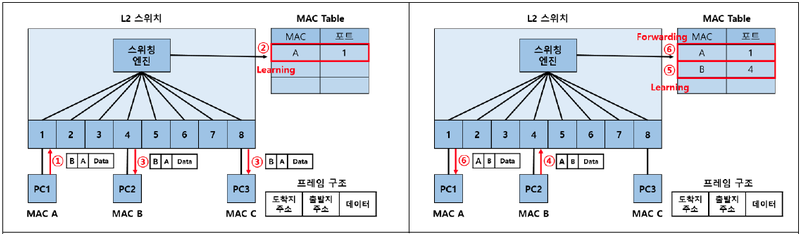
\includegraphics[width=.65\textwidth]{image/week05/4-1.png}
		\caption{\small L2 Switch}
		\vspace{-10pt}
    \end{figure}
    
    위의 그림과 같이 MAC Table에 출발지/목적지 주소 정보가 없는 Frame이 들어왔을때의 동작을 알아보자. \\
    \begin{enumerate}
        \item 1번 포트에 연결된 PC1(MAC 주소 A)에서 MAC 주소 B로 Frame을 전송한다.
        \item 출발지 PC1의 MAC 주소 A와 포트 번호 1을 매칭하여 MAC Table에 저장한다. (Learning)
        \item 목적지 MAC 주소 B가 MAC Table에 없으므로 전체 포트에 Frame을 복사, 전송한다. (Flooding)
        \item PC2(MAC 주소 B)에서 MAC 주소 A로 Frame을 전송한다.
        \item 출발지 MAC 주소 B와 포트 번호 4를 매칭하여 MAC Table에 저장한다. (Learning)
        \item 목적지 MAC 주소 A가 MAC Table에 있으므로, Frame을 Flooding 없이 포트 1로만 전달한다. (Forwarding)
    \end{enumerate}
\newpage